\documentclass[11pt,a4paper]{article}

\usepackage[left=2cm, right=2cm, top=2cm, bottom=2cm]{geometry}
\usepackage{graphicx}
\usepackage{mathtools}
\usepackage{amssymb}
\usepackage{hyperref}
\usepackage{siunitx}
\usepackage[version=4]{mhchem}


\title{xxx: Supporting information}
\author{Pierre Beaujean}
\begin{document}
\maketitle


\renewcommand{\thetable}{S\arabic{table}}
\renewcommand{\thefigure}{S\arabic{figure}}

\begin{figure}[!h]
	\centering
	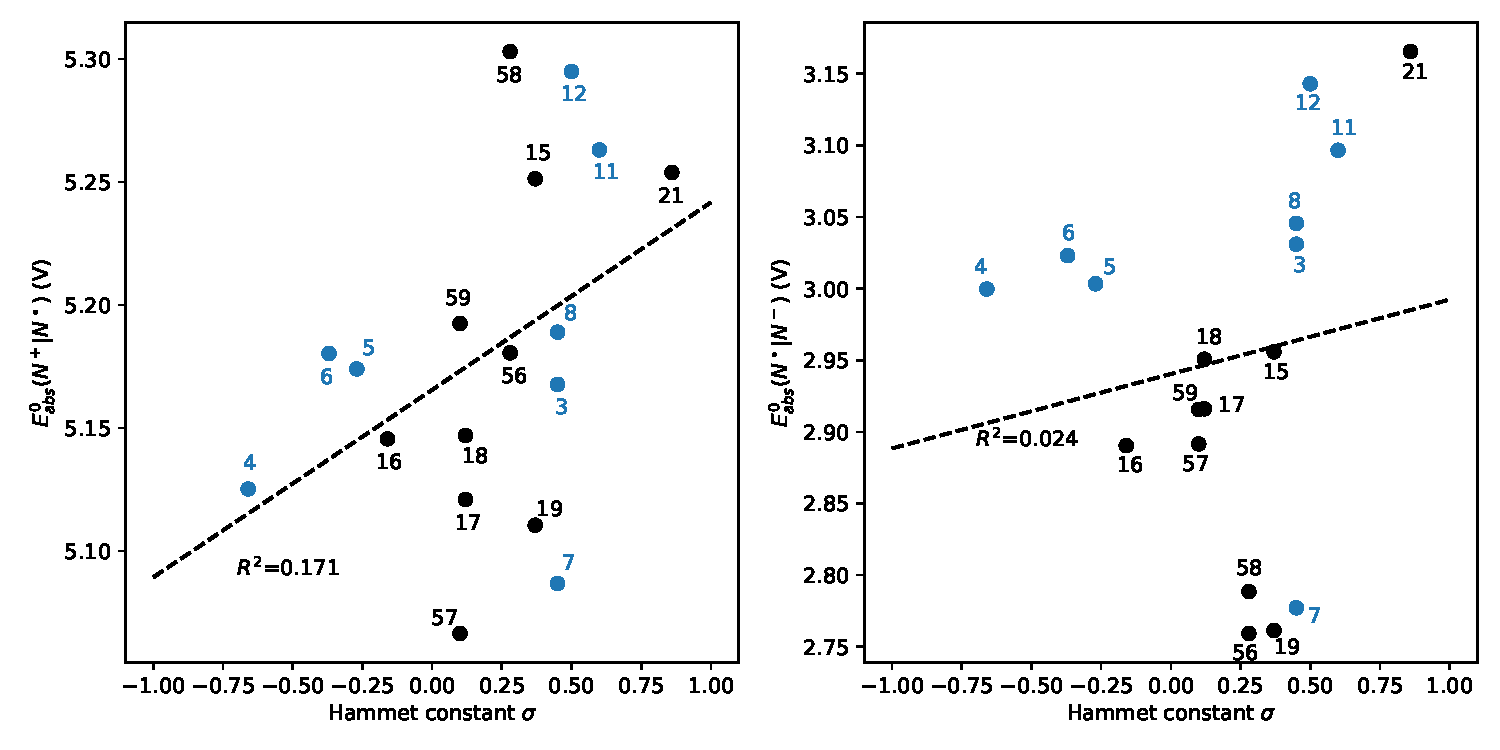
\includegraphics [width=\linewidth]{FigureS1}
	\caption{Evolution of the Born solvatation energy, $\Delta G^\star_{Born}$ (computed with Eq.~(4) of the main text) with the dielectric constant of the solvent (left) for different spherical cavities ($a$) and of the Debye-Huckel correction, $\Delta G^\star_{DH}$  (computed with Eq.~(5) of the main text) with the concentration in electrolyte, $[X]$ (right) in water and acetontrile.}
\end{figure}

\begin{figure}[!h]
\centering
\includegraphics [width=.5\linewidth]{FigureS2}
\caption{Impact of the concentration of electrolyte on the formal oxidation (plain lines, computed with Eq.~(9) of the main text) and reduction (dashed lines, computed with Eq.~(10) of the main text) potentials, $E^f_{abs}$, considering a fictitious case where $E^0_{abs} = \SI{0}{\volt}$.}
\end{figure}

\begin{figure}[!h]
\centering
\includegraphics [width=.7\linewidth]{FigureS3}
\caption{Evolution of the pairing energy, $\Delta G^\star_{pair}$ (computed with Eq.~(11) of the main text) between two ions, with the ratio between the radii of the two ions ($\chi$) and for increasing dipole cavity shapes ($s_2$). Their charge is set to 1 and -1, and two possible scaling for  the close contact distance is used ($s_1$, left and right). The equilibrium constant, $K_{pair} = e^{-\frac{\Delta G^\star_{pair}}{RT}}$, is reported. }
\end{figure}

\begin{figure}[!h]
	\centering
	\includegraphics [width=\linewidth]{FigureS4}
	\caption{Correlation between absolute oxidation (left) and reduction (right) and the Hammet constant of their substituent for compounds of the P5O (black markers) and P6O (blue markers) families.}
\end{figure}

\begin{figure}[!h]
\centering
\includegraphics [width=\linewidth]{FigureS5}
\caption{Difference between the oxygen of the nitroxide redox center ($>$\ce{N=O}) and the center of the counteranion (\ce{A-}, $d_{OX}$) or countercation (\ce{C+}, $d_{red}$) as measured on the geometries optimized at the $\omega$B97X-D/6-311+G(d) level in water (top) and acetonitrile (bottom) using SMD.}
\end{figure}

\begin{figure}[!h]
\centering
\includegraphics [width=\linewidth]{FigureS6}
\caption{Value of the complexation free Gibs energy change for $K_{01}$ (round markers, $\bullet$) and $K_{21}$ (square markers, $\blacksquare$), as computed at the $\omega$B97X-D/6-311+G(d) level in water (top) and acetonitrile (bottom) using SMD at two concentration: $[X]=\SI{1}{\mole\per\liter}$ (filled markers) and  $[X]=\SI{0.1}{\mole\per\liter}$ (empty markers). }
\end{figure}
	
\end{document}